%%%%%%%%%%%%%%%%%%%%%%%%%%%%%%%%%%%%%%%%%%%%%%%%%%%%%%%             
%%         Este template foi adaptado por:           %%
%%                 Oton Crispim Braga                %%
%%    Bacharel em Ciência da Computação - IFCE       %%  
%%  Mestrando em Ciência da Computação - UFERSA/UERN %%
%%                                                   %%
%%                                                   %%
%%                                                   %%
%%                                                   %%
%%  A maior parte deste template foi recuperada      %%
%%         do trabalho desenvolvido por:             %%
%%                                                   %%        
%%            Ednardo Moreira Rodrigues              %%
%%       (Doutor em Engenharia Elétrica - UFC)       %%
%%                      &                            %%
%%            Alan Batista de Oliveira               %%
%%           (Engenheiro Eletricista - UFC)          %%
%%                                                   %%
%% Revisão:                                          %%
%%                                                   %%
%% - Francisco Edvander Pires Santos;                %%
%% - Juliana Soares Lima;                            %%
%% - Izabel Lima dos Santos;                         %%
%% - Kalline Yasmin Soares Feitosa.                  %%
%% - Eliene Maria Vieira de Moura;                   %%
%%                                                   %%
%% Colaboradores                                     %%
%%                                                   %%
%% -Andrei Bosco Bezerra Torres                      %% 
%% (Professor - Sistemas e Mídias Digitais -         %%
%% Instituto Universidade Virtual - UFC)             %%
%% Tiago ALves Lima                                  %% 
%% (Aluno de Mestrado em Eng. Elétrica)              %%
%%                                                   %%
%% Grande parte do trabalho foi adaptado do template %%
%% da UECE elaborado por:                            %%
%% Thiago Nascimento  (UECE)                         %%
%% Project available on:                             %%
%% https://github.com/thiagodnf/uecetex2             %%
%%                                                   %%
%% "Dúvidas, esclarecimentos ou sugestões podem ser  %%
%% enviadas para o seguinte e-mail:                  %%
%%                                                   %%
%%             atendimentobch@ufc.br                 %%
%%                                                   %%
%% As últimas atualizações estão descritas no inicio %%
%% do arquivo "README.md".                           %%
%%                                                   %%
%%%%%%%%%%%%%%%%%%%%%%%%%%%%%%%%%%%%%%%%%%%%%%%%%%%%%%%

\documentclass[        
    a4paper,          % Tamanho da folha A4
    12pt,             % Tamanho da fonte 12pt
    chapter=TITLE,    % Todos os capitulos devem ter caixa alta
    section=Title,    % Todas as secoes devem ter caixa alta somente na primeira letra
    subsection=Title, % Todas as subsecoes devem ter caixa alta somente na primeira letra
    oneside,          % Usada para impressao em apenas uma face do papel
    english,          % Hifenizacoes em ingles
    spanish,          % Hifenizacoes em espanhol
    brazil,           % Ultimo idioma eh o idioma padrao do documento
    fleqn             % Comente esta linha se quiser centralizar as equacoes. Comente também a linha 65 abaixo
]{abntex2}

%%%%%%%%%%%%%%%%%%%%%%%%%%%%%%%%%%%%%%%%%%%%%%%%%%%%%%%             
%%         Este template foi adaptado por:           %%
%%                 Oton Crispim Braga                %%
%%    Bacharel em Ciência da Computação - IFCE       %%  
%%  Mestrando em Ciência da Computação - UFERSA/UERN %%
%%                                                   %%
%%                                                   %%
%%                                                   %%
%%                                                   %%
%%  A maior parte deste template foi recuperada      %%
%%         do trabalho desenvolvido por:             %%
%%                                                   %%        
%%            Ednardo Moreira Rodrigues              %%
%%       (Doutor em Engenharia Elétrica - UFC)       %%
%%                      &                            %%
%%            Alan Batista de Oliveira               %%
%%           (Engenheiro Eletricista - UFC)          %%
%%                                                   %%
%% Revisão:                                          %%
%%                                                   %%
%% - Francisco Edvander Pires Santos;                %%
%% - Juliana Soares Lima;                            %%
%% - Izabel Lima dos Santos;                         %%
%% - Kalline Yasmin Soares Feitosa.                  %%
%% - Eliene Maria Vieira de Moura;                   %%
%%                                                   %%
%% Colaboradores                                     %%
%%                                                   %%
%% -Andrei Bosco Bezerra Torres                      %% 
%% (Professor - Sistemas e Mídias Digitais -         %%
%% Instituto Universidade Virtual - UFC)             %%
%% Tiago ALves Lima                                  %% 
%% (Aluno de Mestrado em Eng. Elétrica)              %%
%%                                                   %%
%% Grande parte do trabalho foi adaptado do template %%
%% da UECE elaborado por:                            %%
%% Thiago Nascimento  (UECE)                         %%
%% Project available on:                             %%
%% https://github.com/thiagodnf/uecetex2             %%
%%                                                   %%
%% "Dúvidas, esclarecimentos ou sugestões podem ser  %%
%% enviadas para o seguinte e-mail:                  %%
%%                                                   %%
%%             atendimentobch@ufc.br                 %%
%%                                                   %%
%% As últimas atualizações estão descritas no inicio %%
%% do arquivo "README.md".                           %%
%%                                                   %%
%%%%%%%%%%%%%%%%%%%%%%%%%%%%%%%%%%%%%%%%%%%%%%%%%%%%%%%

% Importações de pacotes
\usepackage[utf8]{inputenc}                         % Acentuação direta
\usepackage[T1]{fontenc}                            % Codificação da fonte em 8 bits
\usepackage{graphicx}                               % Inserir figuras
\usepackage{amsfonts, amssymb, amsmath}             % Fonte e símbolos matemáticos
\usepackage{booktabs}                               % Comandos para tabelas
\usepackage{verbatim}                               % Texto é interpretado como escrito no documento
\usepackage{multirow, array}                        % Múltiplas linhas e colunas em tabelas
\usepackage{indentfirst}                            % Endenta o primeiro parágrafo de cada seção.
\usepackage{listings}                               % Utilizar codigo fonte no documento
\usepackage{xcolor}
\usepackage{microtype}                              % Para melhorias de justificação?
\usepackage[portuguese,ruled,lined]{algorithm2e}    % Escrever algoritmos
\usepackage{algorithmic}                            % Criar Algoritmos  
%\usepackage{float}                                 % Utilizado para criação de floats
\usepackage{amsgen}
\usepackage{lipsum}                                 % Usar a simulação de texto Lorem Ipsum
%\usepackage{titlesec}                              % Permite alterar os títulos do documento
\usepackage{tocloft}                                % Permite alterar a formatação do Sumário
\usepackage{etoolbox}                               % Usado para alterar a fonte da Section no Sumário
\usepackage[nogroupskip,nonumberlist]{glossaries}   % Permite fazer o glossario

\usepackage[font=singlespacing,format=plain,justification=justified,skip=0pt,singlelinecheck = false]{caption}            % Altera o comportamento da tag caption

\usepackage[alf, abnt-emphasize=bf, recuo=0cm, abnt-etal-cite=2, abnt-etal-list=0, abnt-etal-text=it]{abntex2cite}  % Citações padrão ABNT
%\usepackage[bottom]{footmisc}                      % Mantém as notas de rodapé sempre na mesma posição
%\usepackage{times}                                 % Usa a fonte Times
%%%%%%%%%%%%%%%%%%% AVISO %%%%%%%%%%%%%%%%%%%%%%%%%%%%%%%%%%%%%%%%
%descomente as duas linhas abaixo para alterar o texto de Times New Roman para Arial:

%\usepackage{helvet}
%\renewcommand{\familydefault}{\sfdefault}  % Usa a fonte Arial              
%%%%%%%%%%%%%%%%%%%%%%%%%%%%%%%%%%%%%%%%%%%%%%%%%%%%%%%%%%%%%%%%%%

\usepackage{mathptmx}         % Usa a fonte Times New Roman			%\usepackage{lmodern}         % Usa a fonte Latin Modern
%\usepackage{subfig}          % Posicionamento de figuras
%\usepackage{scalefnt}        % Permite redimensionar tamanho da fonte
%\usepackage{color, colortbl} % Comandos de cores
%\usepackage{lscape}          % Permite páginas em modo "paisagem"
%\usepackage{ae, aecompl}     % Fontes de alta qualidade
%\usepackage{picinpar}        % Dispor imagens em parágrafos
%\usepackage{latexsym}        % Símbolos matemáticos
%\usepackage{upgreek}         % Fonte letras gregas
\usepackage{appendix}         % Gerar o apendice no final do documento
\usepackage{paracol}          % Criar paragrafos sem identacao
\usepackage{lib/ppgcctex}	      % Biblioteca com as normas da UFC para trabalhos academicos
\usepackage{pdfpages}         % Incluir pdf no documento
\usepackage{amsmath}          % Usar equacoes matematicas

% importar meu pacotes
\usepackage{setspace}

\makeglossaries % Organiza e gera a lista de abreviaturas, simbolos e glossario
\makeindex      % Gera o Indice do documento         




\setlength{\mathindent}{0pt} %Complementa o alinhamento de equações para totalmente a esquerda.

%%%%%%%%%%%%%%%%%%%%%%%%%%%%%%%%%%%%%%%%%%%%%%%%%%%%%
%%                     ATENCAO                     %%
%%%%%%%%%%%%%%%%%%%%%%%%%%%%%%%%%%%%%%%%%%%%%%%%%%%%%
%  Qual e o nivel do trabalho academico que voce esta 
% escrevendo? Retire o simbolo "%" apenas de um dos 
% quatro topicos abaixo refente ao nível do seu traba
% -lho.

% \trabalhoacademico{tccgraduacao}
%\trabalhoacademico{tccespecializacao}
\trabalhoacademico{dissertacao}
%\trabalhoacademico{tese}

%%%%%%%%%%%%%%%%%%%%%%%%%%%%%%%%%%%%%%%%%%%%%%%%%%%%%

% Define se o trabalho e uma qualificacao
% Coloque 'nao' para versao final do trabalho

\ehqualificacao{sim}

% Remove as bordas vermelhas e verdes do PDF gerado
% Coloque 'sim' pare remover

\removerbordasdohyperlink{sim} 

% Adiciona a cor Azul a todos os hyperlinks

\cordohyperlink{nao}

%%%%%%%%%%%%%%%%%%%%%%%%%%%%%%%%%%%%%%%%%%%%%%%%%%%%%
%%         Informacao sobre a instituicao          %%
%%%%%%%%%%%%%%%%%%%%%%%%%%%%%%%%%%%%%%%%%%%%%%%%%%%%%

\ies{Universidade Federal Rural do Semi-Árido}
\iesdois{Universidade Estadual do Rio Grande do Norte}
\iessigla{UFERSA}
\iessigladois{UERN}
\centro{Centro de Xxxxxxxx}
\departamento{Departamento de Xxxxxxxxx}

%%%%%%%%%%%%%%%%%%%%%%%%%%%%%%%%%%%%%%%%%%%%%%%%%%%%%
%%        Informacao para TCC de Graduacao         %%
%%%%%%%%%%%%%%%%%%%%%%%%%%%%%%%%%%%%%%%%%%%%%%%%%%%%%

\graduacaoem{Engenharia Xxxxxxx}
\habilitacao{bacharel} % Ou licenciado(a)

% AVISO: Caso necessario alterar o texto de apresenta-
% cao da Especializacao, ir a pasta "lib", arquivo 
% "ufctex.sty" na linha 502.


%%%%%%%%%%%%%%%%%%%%%%%%%%%%%%%%%%%%%%%%%%%%%%%%%%%%%
%%     Informacao para TCC de Especializacao       %%
%%%%%%%%%%%%%%%%%%%%%%%%%%%%%%%%%%%%%%%%%%%%%%%%%%%%%

\especializacaoem{Yyyyyyyyy}

% AVISO: Caso necessario alterar o texto de apresenta-
% cao da Especializacao, ir a pasta "lib", arquivo 
% "ufctex.sty" na linha 507.

%%%%%%%%%%%%%%%%%%%%%%%%%%%%%%%%%%%%%%%%%%%%%%%%%%%%%
%%         Informacao para Dissertacao             %%
%%%%%%%%%%%%%%%%%%%%%%%%%%%%%%%%%%%%%%%%%%%%%%%%%%%%%

\programamestrado{Programa de Pós-Graduação em Ciências da Computação}
\nomedomestrado{Mestrado Acadêmico em Xxxxxxx} % opicional
\mestreem{Ciência da Computação} 
\areadeconcentracaomestrado{Engenharia Xxxxxx} % opicional

% AVISO: Caso necessario alterar o texto de apresenta-
% cao da dissertacao, ir a pasta "lib", arquivo 
% "ufctex.sty" na linha 511.

%%%%%%%%%%%%%%%%%%%%%%%%%%%%%%%%%%%%%%%%%%%%%%%%%%%%%
%%               Informação para Tese              %%
%%%%%%%%%%%%%%%%%%%%%%%%%%%%%%%%%%%%%%%%%%%%%%%%%%%%%

\programadoutorado{Programa de Pós-Graduação em Xxxxxx}
\nomedodoutorado{Doutorado em Xxxxxxx}
\doutorem{Engenharia Xxxxxx}
\areadeconcentracaodoutorado{Xxxxxxx}

% AVISO: Caso necessario alterar o texto de apresenta-
% cao da tese, ir a pasta "lib", arquivo "ufctex.sty" 
% na linha 515.

%%%%%%%%%%%%%%%%%%%%%%%%%%%%%%%%%%%%%%%%%%%%%%%%%%%%%
%%      Informacoes relacionadas ao trabalho       %%
%%%%%%%%%%%%%%%%%%%%%%%%%%%%%%%%%%%%%%%%%%%%%%%%%%%%%

\autor{Nome Sobrenome} 
\titulo{Título do Trabalho}
\data{2019}
\local{Mossoró}

% Exemplo: \dataaprovacao{01 de Janeiro de 2012}
\dataaprovacao{}

%%%%%%%%%%%%%%%%%%%%%%%%%%%%%%%%%%%%%%%%%%%%%%%%%%%%%
%%           Informação sobre o Orientador         %%
%%%%%%%%%%%%%%%%%%%%%%%%%%%%%%%%%%%%%%%%%%%%%%%%%%%%%

\orientador{Prof. Dr. Xxxxxxx Xxxxxx Xxxxxxx}
\orientadories{UFERSA}
\orientadorcentro{Centro de Ciências e Tecnologia (CCT)} % opicional
\orientadorfeminino{nao} % Coloque 'sim' se for do sexo feminino

%%%%%%%%%%%%%%%%%%%%%%%%%%%%%%%%%%%%%%%%%%%%%%%%%%%%%
%%          Informação sobre o Coorientador        %%
%%%%%%%%%%%%%%%%%%%%%%%%%%%%%%%%%%%%%%%%%%%%%%%%%%%%%

% Deixe o nome do coorientador em branco para remover do documento

\coorientador{}
\coorientadories{SIGLA}
\coorientadorcentro{Centro do Coorientador (SIGLA)} % opicional
\coorientadorfeminino{nao} % Coloque 'sim' se for do sexo feminino

%%%%%%%%%%%%%%%%%%%%%%%%%%%%%%%%%%%%%%%%%%%%%%%%%%%%%
%%              Informação sobre a banca           %%
%%%%%%%%%%%%%%%%%%%%%%%%%%%%%%%%%%%%%%%%%%%%%%%%%%%%%

% Atenção! Deixe em branco o nome do membro da banca para remover da folha de aprovacao

% Exemplo de uso:
% \membrodabancadois{Prof. Dr. Fulano de Tal}
% \membrodabancadoisies{Universidade Federal do Ceará - UFC}

\membrodabancadois{Prof. Dr. Xxxxxxx Xxxxxx Xxxxxxx}
\membrodabancadoiscentro{}
\membrodabancadoisies{SIGLA}
\membrodabancatres{Prof. Dr. Xxxxxxx Xxxxxx Xxxxxxx}
\membrodabancatrescentro{}
\membrodabancatresies{SIGLA}
\membrodabancaquatro{Prof. Dr. Xxxxxxx Xxxxxx Xxxxxxx}
\membrodabancaquatrocentro{}
\membrodabancaquatroies{SIGLA}
\membrodabancacinco{Prof. Dr. Xxxxxxx Xxxxxx Xxxxxxx}
\membrodabancacincocentro{Teste}
\membrodabancacincoies{Universidade do Membro da Banca Cinco (SIGLA)}
\membrodabancaseis{Prof. Dr. Xxxxxxx Xxxxxx Xxxxxxx}
\membrodabancaseiscentro{}
\membrodabancaseisies{Universidade do Membro da Banca Seis (SIGLA)}

\begin{document}	

	% Elementos pré-textuais
	\imprimircapa
	\imprimirfolhaderosto{}
% 	\imprimirfichacatalografica{1-pre-textuais/ficha-catalografica} %  gerada pela biblioteca 
	%\imprimirerrata{elementos-pre-textuais/errata}
	\imprimirfolhadeaprovacao % desnecessario para qualificacao
	\imprimirdedicatoria{1-pre-textuais/dedicatoria}
	\imprimiragradecimentos{1-pre-textuais/agradecimentos}
	\imprimirepigrafe{1-pre-textuais/epigrafe}
	\imprimirresumo{1-pre-textuais/resumo}
	\imprimirabstract{1-pre-textuais/abstract}
	\renewcommand*\listfigurename{Lista de Figuras} %Se você comentar esta linha o título da lista fica: LISTA DE ILUSTRAÇÕES
	\imprimirlistadeilustracoes
	\imprimirlistadetabelas
	%\imprimirlistadequadros
	%\imprimirlistadealgoritmos
	%\imprimirlistadecodigosfonte
	\imprimirlistadeabreviaturasesiglas
	\imprimirlistadesimbolos{1-pre-textuais/lista-de-simbolos}   
	\imprimirsumario
	
	\setcounter{table}{0}% Deixe este comando antes da primeira tabela.
	
	%Elementos textuais
	\textual
	\chapter{Introdução}
\label{cap:introducao}

%Para começar a usar este \textit{template}, na plataforma \textit{ShareLatex}, vá nas opções (três barras vermelhas horizontais) no canto esquerdo superior da tela e clique em "Copiar Projeto" e dê um novo nome para o projeto. 

Para começar a utilizar este \textit{template}, siga o tutorial clicando no seguinte \textit{link}:
\url{http://www.biblioteca.ufc.br/images/arquivos/instrucoes_modelos/tutorial_sharelatex.pdf}

Neste \textit{template}, o autor irá encontrar diversas instruções e exemplos dos recursos do uso do \LaTeX~na plataforma \textit{ShareLatex}. O \LaTeX~foi desenvolvido, inicialmente, na década de 80, por Leslie Lamport e é utilizado amplamente na produção de textos matemáticos e científicos, devido a sua alta qualidade tipográfica \cite{goossens1994latex}. 

O \textit{ShareLatex} é uma plataforma \textit{online} que pode ser acessado por meio de qualquer navegador de internet até mesmo de um \textit{smartphone}. Essa plataforma dispensa a instalação de aplicativos no computador para desenvolver trabalhos em \LaTeX. Também, não é necessário instalar \textit{packages}, ou seja, pacotes que permitem diferentes efeitos na formatação e no visual do trabalho. Todos os \textit{packages} que este \textit{template} utiliza são encontrados \textit{online}. 

Apresentam-se, também, neste modelo, algumas orientações de como desenvolver um trabalho acadêmico. Entretanto, este arquivo deve ser editado pelo autor de acordo com o seu trabalho sendo que a formatação já está de acordo com o aceito pela Universidade Federal do Ceará.  

A introdução, tem como finalidade, dar ao leitor uma visão concisa do tema investigado, ressaltando-se o assunto de forma delimitada, ou seja, enquadrando-o sob a perspectiva de uma área do conhecimento, de forma que fique evidente sobre o que se está investigando; a justificativa da escolha do tema; os objetivos do trabalho; o objeto de pesquisa que será investigado. Observe que não se divide a introdução em seções, mas a mesma informa como o trabalho ao todo está organizado.



%Testando o símbolo $\symE$

%\lipsum[5]  % Simulador de texto, ou seja, é um gerador de lero-lero.

%	\begin{alineas}
%		\item Lorem ipsum dolor sit amet, consectetur adipiscing elit. Nunc dictum sed tortor nec viverra.
%		\item Praesent vitae nulla varius, pulvinar quam at, dapibus nisi. Aenean in commodo tellus. Mauris molestie est sed justo malesuada, quis feugiat tellus venenatis.
%		\item Praesent quis erat eleifend, lacinia turpis in, tristique tellus. Nunc dictum sed tortor nec viverra.
%		\item Mauris facilisis odio eu ornare tempor. Nunc dictum sed tortor nec viverra.
%		\item Curabitur convallis odio at eros consequat pretium.
%	\end{alineas}
	

	

	\chapter{Título do segundo capítulo}
\label{cap:fundamentacao-teorica}

Alguns autores preferem fazer uma ``fundamentação teórica'' no segundo capítulo, outros, preferem fazer uma ``revisão da literatura''. Entretanto, isto é particular de cada trabalho e o autor deve escolher o título mais adequado para o capítulo. Consultar o orientador é importante para determinar o título apropriado.

Evite começar da seção secundária, ou seja, não passe direto do título do capítulo para o título da seção secundária. Escreva um texto para introduzir as seções subsequentes. Lembre-se de utilizar primeira letra maiúscula quando estiver se referindo a um objeto com numeração específica como capítulo, seção, subseção, figura, tabela, quadro, equação, normalmente, se escreve a primeira letra maiúscula da palavra do objeto seguido do \textit{label}. Por exemplo, a Seção \ref{sec:citacoes} explica como fazer citações bibliográficas. Observe no código fonte deste texto como foi feita a referência cruzada. Isso permite enumerar a seção do modo automático o que facilita caso novas seções sejam criadas.  

\section{Citações bibliográficas}\label{sec:citacoes}

    Esta frase mostra como citar um livro sobre descargas atmosféricas \cite{rakov2003lightning}. Também podem ser citados \textit{sites} como \citeonline{elat2015densidade}. Você precisa escrever o código da referência no arquivo "referencia.bib" dentro da pasta "elementos-pos-textuais". Veja esse, onde estão alguns exemplos que já foram testados.        

    Referenciando outro livro \cite{LangtangenLogg2017}. Texto texto texto texto texto texto texto texto texto texto texto texto texto texto texto texto texto texto texto. Texto texto texto texto texto texto texto texto texto texto texto texto texto texto texto texto texto texto texto. Texto texto texto texto texto texto texto texto texto texto texto texto texto texto texto texto texto texto texto. Texto texto texto texto texto texto texto texto texto texto texto texto texto texto texto texto texto texto texto.

    Referenciando outro site \cite{secretaria1999}. Texto texto texto texto texto texto texto texto texto texto texto texto texto texto texto texto texto texto texto. Texto texto texto texto texto texto texto texto texto texto texto texto texto texto texto texto texto texto texto. Texto texto texto texto texto texto texto texto texto texto texto texto texto texto texto texto texto texto texto. Texto texto texto texto texto texto texto texto texto texto texto texto texto texto texto texto texto texto texto. Citando uma norma \cite{NBR10520:2002}.
        
    Citação de duas referências que concordam entre si \cite{Almeida2018,Gondim2017}. Texto texto texto texto texto texto texto texto texto texto texto texto texto texto texto texto texto texto texto. Texto texto texto texto texto texto texto texto texto texto texto texto texto texto texto texto texto texto texto. Texto texto texto texto texto texto texto texto texto texto texto texto texto texto texto texto texto texto texto. Texto texto texto texto texto texto texto texto texto texto texto texto texto texto texto texto texto texto texto texto texto texto texto texto texto texto. Citando um manual \cite{manuais1989}. 
        
    Outro tipo de citação é a citação literal ou direta com mais de três linhas. Este tipo de citação deve ser destacada com recuo de $4~cm$ da margem esquerda com letra menor (tamanho 10), sem aspas e com espaçamento simples.  Para exemplificar esse tipo de citação, considere a afirmação de \citeonline{feitosa2016}:
    \begin{citacao}
        A cultura é o processo através do qual o homem cria o algo onde antes imperava o nada. Esse algo é toda complexidade de criações simbólicas, de sentidos e significados que damos às coisas e ao mundo. Um ``algo'' que não se sustenta se não se entender os processos culturais como mecanismos de mediação entre nós e os fenômenos. Assim, mais do que apenas um elemento da comunicação, a mediação é, por excelência, cultural. As diversas modalidades de mediação são apenas sotaques diferenciados dessa mediação cultural. Assim é a mediação informacional.
    \end{citacao}
        
    A afirmação do parágrafo anterior também pode ser reproduzida com a citação na final como mostra o exemplo a seguir: 
    \begin{citacao}
        A cultura é o processo através do qual o homem cria o algo onde antes imperava o nada. Esse algo é toda complexidade de criações simbólicas, de sentidos e significados que damos às coisas e ao mundo. Um “algo” que não se sustenta se não se entender os processos culturais como mecanismos de mediação entre nós e os fenômenos. Assim, mais do que apenas um elemento da comunicação, a mediação é, por excelência, cultural. As diversas modalidades de mediação são apenas sotaques diferenciados dessa mediação cultural. Assim é a mediação informacional. \cite{feitosa2016}.
    \end{citacao}
        
%Mais exemplos e opções de citações podem ser encontradas em:
%        https://en.wikibooks.org/wiki/LaTeX/Bibliography_Management
%        https://github.com/cfgnunes/latex-cefetmg/blob/master/latex-cefetmg/03-elementos-pos-textuais/apendices.tex            

\section{Inserindo figuras}\label{sec:figuras}
    
    A Figura \ref{fig:reitoria} apresenta a fotografia da reitoria da Universidade Federal do Ceará. Observe a estrutura do código para ver como inserir figuras. No título, comece especificando o tipo de figura. Por exemplo, fotografia, desenho, diagrama, fluxograma, gráfico e etc. O espaçamento entre linhas no título é de $1~pt$ (espaçamento simples), apenas a primeira letra da frase é maiúscula. As demais palavras são escritas com letra maiúsculas somente quando são nomes próprios e não há ponto final. 
    
    As margens do título da figura são delimitadas pelo tamanho da figura. Por isso, procure ajustar o tamanho da figura para preencher a largura delimitada pelas margens esquerda e direita da página que possui $16~cm$ de largura. Não esqueça de indicar fonte da figura. O autor deve evitar deixar figuras pequenas menores do que $7~cm$ de largura.
    
    A posição da figura deve ser o mais próximo logo após ter sido chamada no texto (a figura nunca deve aparecer antes de ter sido anunciada no texto). 
    
    %troque h pelo b ou t para mudar a posição da figura.
 	\begin{figure}[h!] 
   	    \captionsetup{width=16cm}%Da mesma largura que a figura
		\Caption{\label{fig:reitoria} Fotografia da reitoria da Universidade Federal do Ceará}
		\UFCfig{}{
			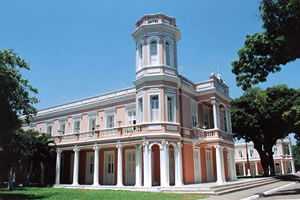
\includegraphics[width=16cm]{figuras/exemplo-1}
		}{
			\Fonte{\citeonline{UFC2012}.}
		}	
	\end{figure}
	
    Texto1 texto texto texto texto texto texto texto texto texto texto texto texto texto texto texto texto texto texto texto texto texto texto texto texto texto texto texto texto texto texto texto texto texto texto texto texto texto texto texto texto texto texto texto texto1.

    Texto2 texto texto texto texto texto texto texto texto texto texto texto texto texto texto texto texto texto texto. Texto texto texto texto texto texto texto texto texto texto texto texto texto texto texto texto texto texto texto2.

    Texto3 texto texto texto texto texto texto texto texto texto texto texto texto texto texto texto texto texto texto. Texto texto texto texto texto texto texto texto texto texto texto texto texto texto texto texto texto texto texto3.

    Texto4 texto texto texto texto texto texto texto texto texto texto texto texto texto texto texto texto texto texto. Texto texto texto texto texto texto texto texto texto texto texto texto texto texto texto texto texto texto texto4.

    A Figura \ref{fig:sondas} Texto texto texto texto texto texto texto texto texto texto texto texto texto texto texto texto texto texto texto. Texto texto texto texto texto texto texto texto texto texto texto texto texto texto texto texto texto texto texto3.

	\begin{figure}[h!]
		\centering
		\captionsetup{width=14cm}%Da mesma largura que a figura
		\Caption{\label{fig:sondas} Gráfico da Atmosfera Superior}	
		\UFCfig{}{
			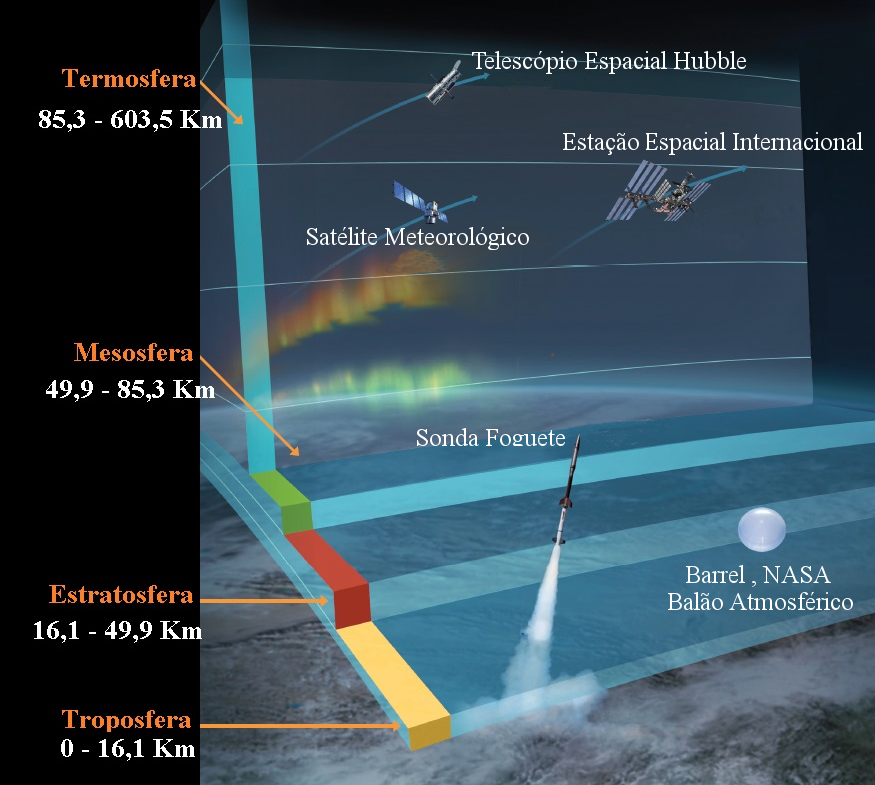
\includegraphics[width=14cm]{figuras/sondas}
		}{
			\Fonte{adaptado da \citeonline{NASA2016}.}}	
	\end{figure}

    Texto5 texto texto texto texto texto texto texto texto texto texto texto texto texto texto texto texto texto texto texto texto texto texto texto texto texto texto texto texto texto texto texto texto texto texto texto texto texto texto texto texto texto texto texto texto5.

    Texto6 texto texto texto texto texto texto texto texto texto texto texto texto texto texto texto texto texto texto texto texto texto texto texto texto texto texto texto texto texto texto texto texto texto texto texto texto texto texto texto texto texto texto texto texto5.

    Texto7 texto texto texto texto texto texto texto texto texto texto texto texto texto texto texto texto texto texto texto texto texto texto texto texto texto texto texto texto texto texto texto texto texto texto texto texto texto texto texto texto texto texto texto texto texto texto texto texto texto texto texto texto texto texto texto texto texto texto texto texto texto texto texto6.

    Evite terminar seções, capítulos e etc com figura. Procure escrever mais.

\section{Inserindo tabelas}\label{sec:tabelas}
    
    A Tabela \ref{tab:exemplo-1}... texto texto texto texto texto texto texto texto texto texto texto texto texto texto texto texto texto texto texto. Texto texto texto texto texto texto texto texto texto texto texto texto texto texto texto texto texto texto texto.
	
	\begin{table}[!h]
	\captionsetup{width=7cm}%Deixe da mesma largura que a tabela
	\Caption{\label{tab:exemplo-1} Um Exemplo de tabela alinhada que pode ser longa ou curta}%
	\IBGEtab{}{%
		\begin{tabular}{ccc}
			\toprule
			Nome & Nascimento & Documento \\
			\midrule \midrule
			Maria da Silva & 11/11/1111 & 111.111.111-11 \\
			Maria da Silva & 11/11/1111 & 111.111.111-11 \\
			Maria da Silva & 11/11/1111 & 111.111.111-11 \\
			\bottomrule
		\end{tabular}%
	}{%
	\Fonte{o autor.}%
	\Nota{esta é uma nota, que diz que os dados são baseados na
		regressão linear.}%
	\Nota[Anotações]{uma anotação adicional, seguida de várias outras.}%
    }
    \end{table}

	%\begin{table}[h!]	
	%	\centering
	%	\Caption{\label{tab:exemplo-1} Exemplo de tabela}	
	%	\UFCtab{}{
	%		\begin{tabular}{cll}
	%			\toprule
	%			Ranking & Exon Coverage & Splice Site Support \\
	%			\midrule \midrule
	%			E1 & Complete coverage by a single transcript & Both splice sites\\
	%			E2 & Complete coverage by more than a single transcript & Both splice sites\\
	%			E3 & Partial coverage & Both splice sites\\
	%			E4 & Partial coverage & One splice site\\
	%			E5 & Complete or partial coverage & No splice sites\\
	%			E6 & No coverage & No splice sites\\
	%			\bottomrule
	%		\end{tabular}
	%	}{
	%	\Fonte{elaborado pelo autor.}
	%}
	%\end{table}

\subsection{Exemplo de subseção} \label{sec:ex_sec}
	
    Texto texto texto texto texto texto texto texto texto texto texto texto texto texto texto texto texto texto texto texto texto texto texto texto texto texto texto texto texto texto texto texto texto texto texto texto texto texto texto texto texto texto texto texto texto.

    %acrlong{DATASUS},\acrlong{DNV},\acrlong{DO},\acrlong{ESF},\acrlong{IBGE},\acrlong{MFC},\acrlong{MI},\acrlong{MS},\acrlong{NV},\acrlong{ODM},\acrlong{OI},\acrlong{OMS},\acrlong{ONU},\acrlong{PNI},\acrlong{PSF},\acrlong{RIPSA},\acrlong{RN},\acrlong{SIM},\acrlong{SINASC},\acrlong{SUS},\acrlong{TMI},\acrlong{TMMFC}


    \begin{alineascomponto}
	    \item Integer non lacinia magna. Aenean tempor lorem tellus, non sodales nisl commodo ut
	    \item Proin mattis placerat risus sit amet laoreet. Praesent sapien arcu, maximus ac fringilla efficitur, vulputate faucibus sem. Donec aliquet velit eros, sit amet elementum dolor pharetra eget
	    \item Integer eget mattis libero. Praesent ex velit, pulvinar at massa vel, fermentum dictum mauris. Ut feugiat accumsan augue, et ultrices ipsum euismod vitae
	    \begin{subalineascomponto}
		    \item Integer non lacinia magna. Aenean tempor lorem tellus, non sodales nisl commodo ut
		    \item Proin mattis placerat risus sit amet laoreet.
	    \end{subalineascomponto}
    \end{alineascomponto}

\subsection{Uso de siglas} \label{sec:siglas}

    Para utilizar siglas, primeiro defina a sigla no arquivo "lista-de-abreviaturas-e-siglas"~ dentro da pasta "1-pre-textuais" com o comando 
    \begin{verbatim}
        \newacronym{ABNT}{ABNT}{Associação Brasileira de Normas Técnicas}
    \end{verbatim}
    Depois chame a sigla com o comando:
    \begin{verbatim}
        \gls{ABNT}
    \end{verbatim}
    Fica assim: \gls{ABNT}. A primeira vez que o comando é usado para uma determinada sigla, aparece o significado por extenso da sigla com a sua abreviação em seguida. A partir da segunda vez que o comando para uma determinada sigla é usado, aparace apenas a sigla. Por exemplo: \gls{ABNT}.  
    
    Veja o código fonte de outros exemplos: Teste de siglas \gls{TEST}, outros exemplos de siglas: \gls{DA}, \gls{MCEG}. 
    Repare que sempre as siglas estão sendo definidas primeiramente no arquivo ``lista-de-abreviaturas-e-siglas''.
	\chapter{Metodologia}
\label{chap:metodologia}

Texto texto texto texto texto texto texto texto texto texto texto texto texto texto texto texto texto texto texto texto texto texto texto texto texto texto texto texto texto texto texto texto texto texto texto texto texto texto texto texto texto texto texto texto texto texto texto texto texto texto texto texto texto texto texto texto texto texto texto texto texto texto texto texto texto texto texto texto texto.

Texto texto texto texto texto texto texto texto texto texto texto texto texto texto texto texto texto texto texto texto texto texto texto texto texto texto texto texto texto texto texto texto texto texto texto texto texto texto texto texto texto texto texto texto texto texto texto texto texto texto texto texto texto texto texto texto texto texto texto texto texto texto texto texto texto texto texto texto texto.

\section{Exemplo de alíneas}\label{sec:exemplo-de-algoritmos-e-figuras}

    Texto texto texto texto texto texto texto texto texto texto texto texto texto texto texto texto texto texto texto texto texto texto texto texto texto texto texto texto texto texto texto texto texto texto texto texto texto texto texto texto texto texto texto texto texto texto texto texto texto texto texto texto texto texto texto texto texto texto texto texto texto texto texto texto texto texto texto texto texto.

    %\begin{algorithm}[h!]
    %	\SetSpacedAlgorithm
    %	\caption{\label{exemplo-de-algoritmo}Como escrever algoritmos no \LaTeX2e}
    %	\Entrada{o proprio texto}
    %	\Saida{como escrever algoritmos com  Latex:}% \LaTeX2e }
    %	\Inicio{
    %		inicialização;
    %		\Repita{fim do texto}{
    %			leia o atual;
    %			\Se{entendeu}{
    %				vá para o proximo\;
    %				próximo se torna o atual;}
    %			\Senao{volte ao início da seção;}
    %		}
    %	}	
    %\end{algorithm}

    Texto texto texto texto texto texto texto texto texto texto texto.

    %\begin{algorithm}[H]
    %	\Entrada{o proprio texto}
    %	\Saida{como escrever algoritmos com \LaTeX2e }
    %	\Inicio{
    %		inicialização\;
    %		\Repita{fim do texto}{
    %			leia o atual\;
    %			\Se{entendeu}{
    %				vá para o próximo\;
    %				próximo se torna o atual\;}
    %			\Senao{volte ao início da seção\;}
    %		}
    %	}
    %	\caption{Exemplo de Algoritmo Versao 02}
    %\end{algorithm}

    %\begin{algorithm}
    %	\begin{algorithmic}
    %	\Entrada{o proprio texto}
    %	\Saida{como escrever algoritmos com \LaTeX2e }	
    %	\end{algorithmic}
    %\end{algorithm}

    Exemplo de alíneas com números:

    \begin{alineascomnumero}
	    \item Texto texto texto texto texto texto texto texto texto texto texto texto .
	    \item Texto texto texto texto texto texto texto texto texto texto texto texto .
	    \item Texto texto texto texto texto texto texto texto texto texto texto texto .
	    \item Texto texto texto texto texto texto texto texto texto texto texto texto .
	    \item Texto texto texto texto texto texto texto texto texto texto texto texto .
	    \item Texto texto texto texto texto texto texto texto texto texto texto texto .
    \end{alineascomnumero}

    Texto texto texto texto texto texto texto texto texto texto texto texto texto texto texto texto texto texto texto texto texto texto texto texto texto texto texto texto texto texto texto texto texto texto texto texto texto texto texto texto texto texto texto texto texto texto texto texto texto texto texto texto texto texto texto texto texto texto texto texto texto texto texto texto texto texto texto texto texto.

    Ou então figuras podem ser incorporadas de arquivos externos, como é o caso da \autoref{fig-grafico-1}. Se a figura que ser incluída se tratar de um diagrama, um gráfico ou uma ilustração que você mesmo produza, priorize o uso de imagens vetoriais no formato PDF. Com isso, o tamanho do arquivo final do trabalho será menor, e as imagens terão uma apresentação melhor, principalmente quando impressas, uma vez que imagens vetorias são perfeitamente escaláveis para qualquer dimensão. Nesse caso, se for utilizar o Microsoft Excel para produzir gráficos, ou o Microsoft Word para produzir ilustrações, exporte-os como PDF e os incorpore ao documento conforme o exemplo abaixo. No entanto, para manter a coerência no uso de software livre (já que você está usando LaTeX e abnTeX),  teste a ferramenta InkScape\index{InkScape}. ao CorelDraw\index{CorelDraw} ou ao Adobe Illustrator\index{Adobe! Illustrator}.  De todo modo, caso não seja possível  utilizar arquivos de imagens como PDF, utilize qualquer outro formato, como JPEG, GIF, BMP, etc.  Nesse caso, você pode tentar aprimorar as imagens incorporadas com o software livre \index{Gimp}Gimp. Ele é uma alternativa livre ao Adobe Photoshop\index{Adobe! Photoshop}.

\section{Usando Fórmulas Matemáticas}

Para escrever um símbolo matemático no texto, escreva símbolo entre cifrões, por exemplo, $\alpha$, $\beta$ e $\gamma$ são símbolo do alfabeto grego. Se você quiser inserir equações enumeradas, siga a estrutura de
\begin{equation}
    \label{eq:indices}
	k_{n+1} = n^2 + k_n^2 - k_{n-1}.
\end{equation}
Observe a pontuação, pois a equação faz parte da frase e do parágrafo. Como a equação faz parte da frase, não se utiliza o \textit{label} numérico \ref{eq:indices}. 

Quando for citar a Equação \ref{eq:indices} novamente no texto, utiliza-se o \textit{label} numérico. Repare que a palavra ``Equação'' foi escrita com ``E'' maiúsculo. 

Um exemplo de equações com frações é dado por
\begin{equation}
	\label{eq:fracao}
		\begin{aligned}
			x = a_0 + \cfrac{1}{a_1
				+ \cfrac{1}{a_2
					+ \cfrac{1}{a_3 + \cfrac{1}{a_4} } } }.
		\end{aligned}
	\end{equation}

Texto texto texto texto texto texto texto texto texto texto texto texto texto texto texto texto texto texto texto texto texto texto texto texto texto texto texto texto texto texto texto texto texto texto texto texto texto texto texto texto texto texto texto texto texto texto texto texto texto texto texto texto texto texto texto texto texto texto texto texto texto texto texto texto texto texto texto texto texto
	\begin{equation}
		\begin{aligned}
			k_{n+1} = n^2 + k_n^2 - k_{n-1}.
		\end{aligned}
	\end{equation}
	
Texto texto texto texto texto texto texto texto texto texto texto texto texto texto texto texto texto texto texto texto texto texto texto texto texto texto texto texto texto texto texto texto texto texto texto texto texto texto texto texto texto texto texto texto texto texto texto texto texto texto texto texto texto texto texto texto texto texto texto texto texto texto texto texto texto texto texto texto texto
	\begin{equation}
	\label{eq:trigo}
		\begin{aligned}
			\cos (2\theta) = \cos^2 \theta - \sin^2 \theta
		\end{aligned}.
	\end{equation}
	
Texto texto texto texto texto texto texto texto texto texto texto texto texto texto texto texto texto texto texto texto texto texto texto texto texto texto texto texto texto texto texto texto texto texto texto texto texto texto texto texto texto texto texto texto texto texto texto texto texto texto texto texto texto texto texto texto texto texto texto texto texto texto texto texto texto texto texto texto texto
	\begin{equation}
	\label{eq:matriz}
		\begin{aligned}
			A_{m,n} =
			\begin{pmatrix}
			a_{1,1} & a_{1,2} & \cdots & a_{1,n} \\
			a_{2,1} & a_{2,2} & \cdots & a_{2,n} \\
			\vdots  & \vdots  & \ddots & \vdots  \\
			a_{m,1} & a_{m,2} & \cdots & a_{m,n}
			\end{pmatrix}
		\end{aligned}.
	\end{equation}

Texto texto texto texto texto texto texto texto texto texto texto texto texto texto texto texto texto texto texto texto texto texto texto texto texto texto texto texto texto texto texto texto texto texto texto texto texto texto texto texto texto texto texto texto texto texto texto texto texto texto texto texto texto texto texto texto texto texto texto texto texto texto texto texto texto texto texto texto texto
	\begin{equation}
	\label{eq:sistema}
		\begin{aligned}
			f(n) = \left\{ 
			\begin{array}{l l}
			n/2 & \quad \text{if $n$ is even}\\
			-(n+1)/2 & \quad \text{if $n$ is odd}
			\end{array} \right.
		\end{aligned}.
	\end{equation}
Texto texto texto texto texto texto texto texto texto texto texto texto texto texto texto texto texto texto texto texto texto texto texto texto texto texto texto texto texto texto texto texto texto texto texto texto texto texto texto texto texto texto texto texto texto texto texto texto texto texto texto texto texto texto texto texto texto texto texto texto texto texto texto texto texto texto texto texto texto

%\section{Usando Algoritmos}

%\begin{algorithm}[h!]
%	\SetSpacedAlgorithm
%	\caption{\label{alg:algoritmo_de_colonica_de_formigas}Algoritmo de Otimização por Colônia de Formiga}
%	\Entrada{Entrada do Algoritmo}
%	\Saida{Saida do Algoritmo}
%	\Inicio{
%		Atribua os valores dos parâmetros\;
%		Inicialize as trilhas de feromônios\;
%		\Enqto{não atingir o critério de parada}{
%			\Para{cada formiga}{
%				Construa as Soluções\;
%			}
%			Aplique Busca Local (Opcional)\;
%			Atualize o Feromônio\;
%		}	
%	}		
%\end{algorithm}

\section{Usando Código-fonte}

Um exemplo de código-fonte, ou código de programação encontra-se no Apendice \ref{ap:A}

 
\section{Usando Teoremas, Proposições, etc}

 Texto texto texto texto texto texto texto texto texto texto texto texto texto texto texto texto texto texto texto texto texto texto texto texto texto.

\begin{teo}[Pitágoras]
	Em todo triângulo retângulo o quadrado do comprimento da
	hipotenusa é igual a soma dos quadrados dos comprimentos dos catetos. Usando o Apêndice \ref{ap:C}
\end{teo}


Texto texto texto texto texto texto texto texto texto texto texto texto texto texto texto.

\begin{teo}[Fermat]
	Não existem inteiros $n > 2$, e $x, y, z$ tais que $x^n + y^n = z$
\end{teo}

Texto texto texto texto texto texto texto texto texto texto texto texto texto texto texto.

\begin{prop}
	Para demonstrar o Teorema de Pitágoras...
\end{prop}

Texto texto texto texto texto texto texto texto texto texto texto texto texto texto texto.

\begin{exem}
	Este é um exemplo do uso do ambiente exem definido acima.
\end{exem}

Texto texto texto texto texto texto texto texto texto texto texto texto texto texto texto.


\begin{xdefinicao}
	Definimos o produto de ...
\end{xdefinicao}

Texto texto texto texto texto texto texto texto texto texto texto texto texto texto texto.

\section{Usando Questões} 

Um exemplo de questionário encontra-se no Apêndice \ref{ap:B}.

%Movido para o Apêndice


	\chapter{Resultados}
\label{chap:resultados}

Texto texto texto texto texto texto texto texto texto texto texto texto texto texto texto texto texto texto texto texto texto texto texto texto texto texto texto texto texto texto texto texto texto texto texto texto texto texto texto texto texto texto texto texto texto texto texto texto texto texto texto texto texto texto texto texto texto texto texto texto texto texto texto texto texto texto texto texto texto.

\section{Resultados do Experimento A}
\label{sec:resultados-do-experimento-a}

Procure deixar as figuras dos resultados o maior possível preenchendo a largura do texto do documento que possui $16~cm$.

\begin{figure}[h!]
        \captionsetup{width=16cm}
		\Caption{\label{fig:tensaoimpedanciahumana} Gráfico de tensão considerando a impedância humana}
		%\centering
		\UFCfig{}{
			\fbox{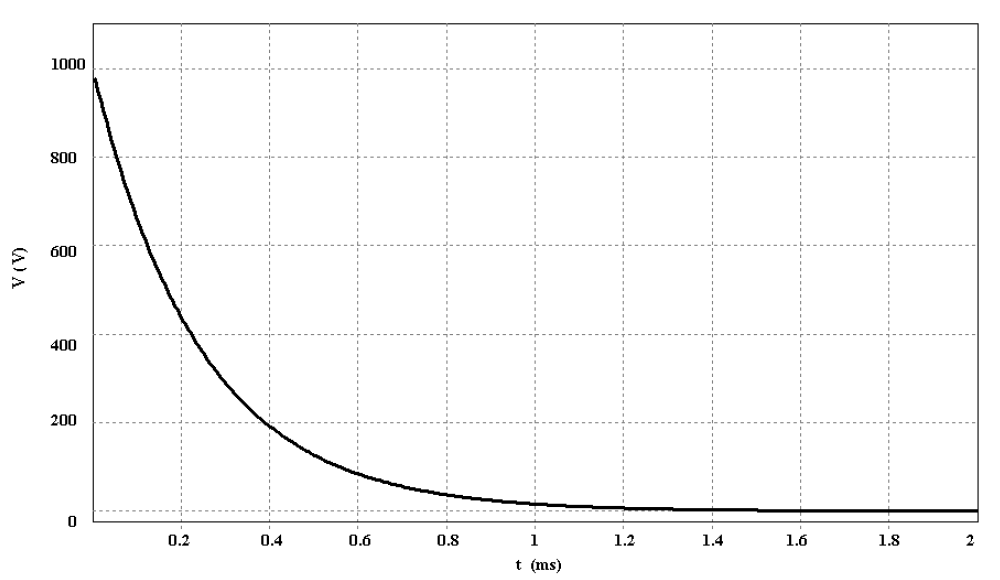
\includegraphics[width=16cm]{figuras/tensaoimpedanciahumana}}
		}{
			\Fonte{elaborado pelo autor (2016).}
		}	
\end{figure}

Texto texto texto texto texto texto texto texto texto texto texto texto texto texto texto texto texto texto texto texto texto texto texto texto texto texto texto texto texto texto texto texto texto texto texto texto texto texto texto texto texto texto texto texto texto texto texto texto texto texto texto texto texto texto texto texto texto texto texto texto texto texto texto texto texto texto texto texto texto.

\begin{figure}[h!]
	\captionsetup{width=16cm}
	\Caption{\label{fig-grafico-1}Produção anual das dissertações de mestrado e teses de doutorado entre os anos de 1990 e 2008}		
	\IBGEtab{}{
		\fbox{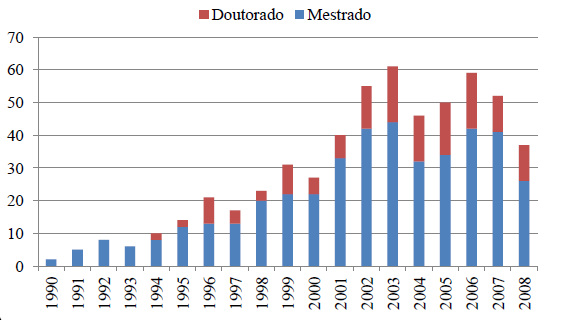
\includegraphics[width=16cm]{figuras/figura-3}}
	}{
	\Fonte{elaborado pelo autor (2016).}
}
\end{figure}

Texto texto texto texto texto texto texto texto texto texto texto texto texto texto texto texto texto texto texto texto texto.

Texto texto texto texto texto texto texto texto texto texto texto texto texto texto texto texto texto texto texto texto texto texto texto texto texto texto texto texto texto texto texto texto texto texto texto texto texto texto texto texto texto texto texto texto texto texto texto texto texto texto texto texto texto texto texto texto texto texto texto texto texto texto texto texto texto texto texto texto texto.

\section{Resultados do Experimento B}
\label{sec:resultados-do-experimento-b}

Texto texto texto texto texto texto texto texto texto texto texto texto texto texto texto texto texto texto texto texto texto texto texto texto texto texto texto texto texto texto texto texto ..

\begin{table}[h!]	
	%\centering
	\captionsetup{width=11.3cm}%ATENÇÃO: Ajuste a largura do título
	\Caption{\label{tab:notas} Notas dos participantes nas avaliações A, B e C}	
	\IBGEtab{}{
		\begin{tabular}{crrr}
			\toprule
			Identificação dos participantes & Avaliação A & Avaliação B &                        Avaliação C \\
			\midrule \midrule
			Participante 1 & 7 & 9 & 10\\
			Participante 2 & 8 & 2 & 1\\
			Participante 3 & 5 & 10 & 6 \\
			Participante 4 & 3 & 1 & 4\\
			Participante 5 & 2 & 4 & 1\\
			Participante 6 & 0 & 7 & 2\\
			\bottomrule
		\end{tabular}
	}{
	\Fonte{elaborado pelo autor (2016).}
}
\end{table}

 Texto texto Referenciando a \autoref{tab:notas}  texto texto texto texto texto texto texto texto texto texto texto texto texto texto texto texto texto texto texto texto texto texto texto texto texto texto texto texto texto texto.Texto texto texto texto texto texto texto texto texto texto texto texto texto texto texto texto texto texto texto texto texto.

Texto texto texto texto texto texto texto texto texto texto texto texto texto texto texto texto texto texto texto texto texto texto texto texto texto texto texto texto texto texto texto texto texto texto texto texto texto texto texto texto texto texto texto texto texto texto texto texto texto texto texto texto texto texto texto texto texto texto texto texto texto texto texto texto texto texto texto texto texto.Texto texto texto texto texto texto texto texto texto texto texto texto texto texto texto texto texto texto texto texto texto texto texto texto texto texto texto texto texto texto texto texto texto texto texto texto texto texto texto texto texto.

Texto texto texto texto texto texto texto texto texto texto texto texto texto texto texto texto texto texto texto texto texto texto texto texto texto texto texto texto texto texto texto texto texto texto texto texto texto texto texto texto texto texto texto texto texto texto texto texto.Texto texto texto texto texto texto texto texto texto texto texto texto texto texto texto texto texto texto texto texto texto.

Texto texto  Referenciando a \autoref{tab:notas}  texto texto texto texto texto texto texto texto texto texto texto texto texto texto texto texto texto texto texto texto texto texto texto texto texto texto texto texto texto texto texto texto texto texto texto texto texto texto texto texto texto texto texto texto texto texto texto texto texto texto texto texto texto texto texto texto texto texto texto texto texto texto texto texto texto texto texto.
	\chapter{Conclusões e Trabalhos Futuros}
\label{chap:conclusoes-e-trabalhos-futuros}

Parte final do texto na qual se apresentam as conclusões apoiadas no desenvolvimento do assunto. É a recapitulação sintética dos resultados obtidos. Pode apresentar recomendações e sugestões para pesquisas futuras.

%\label{sec:contribuicoes-do-trabalho}



%\label{sec:limitacoes}








	
	%Elementos pós-textuais	
	\bibliography{3-pos-textuais/referencias}
%	\imprimirglossario	
	\imprimirapendices
		% Adicione aqui os apendices do seu trabalho
		\apendice{Exemplo de apêndice}
\label{ap:A}

Um apêndice é um documento elaborado pelo autor, diferentemente do anexo. Geralmente, se coloca como apêndice, questionários, códigos de programação, tabelas que tomariam muito espaço no meio do trabalho. Artigos, resumos ou qualquer publicação relacionada ao trabalho podem ser utilizados como apêndice.
		\apendice{Questionário utilizado para...}
\label{ap:B}

\begin{questao}
	\item Esta é a primeira questão com alguns itens:
		\begin{enumerate}
			\item Este é o primeiro item
			\item Segundo item
		\end{enumerate}
	\item Esta é a segunda questão:
		\begin{enumerate}
			\item Este é o primeiro item
			\item Segundo item
		\end{enumerate}
	\item Lorem ipsum dolor sit amet, consectetur adipiscing elit. Nunc dictum sed tortor nec viverra. consectetur adipiscing elit. Nunc dictum sed tortor nec viverra.
		\begin{enumerate}
			\item consectetur
			\item adipiscing
			\item Nunc
			\item dictum
		\end{enumerate}
\end{questao}

		\apendice{Códigos-fontes utilizados para...}
\label{ap:C}

\lstinputlisting[language=C++,caption={Hello World em C++}]{figuras/main.cpp}


\begin{lstlisting}[language=Java,caption={Hello World em Java}]
public class HelloWorld {
	public static void main(String[] args) {
		System.out.println("Hello World!");
	}
}
\end{lstlisting}


		\apendice{\textit{IEEE CEFC 2016}}
\label{ap:D}

\textit{Digest} submetido ao \textit{The 17th Biennial Conference on Eletromagnetic Field Computation, Miami FL - NOV 13-16, 2016, USA}.

%Código fonte para inserir um arquivo em PDF
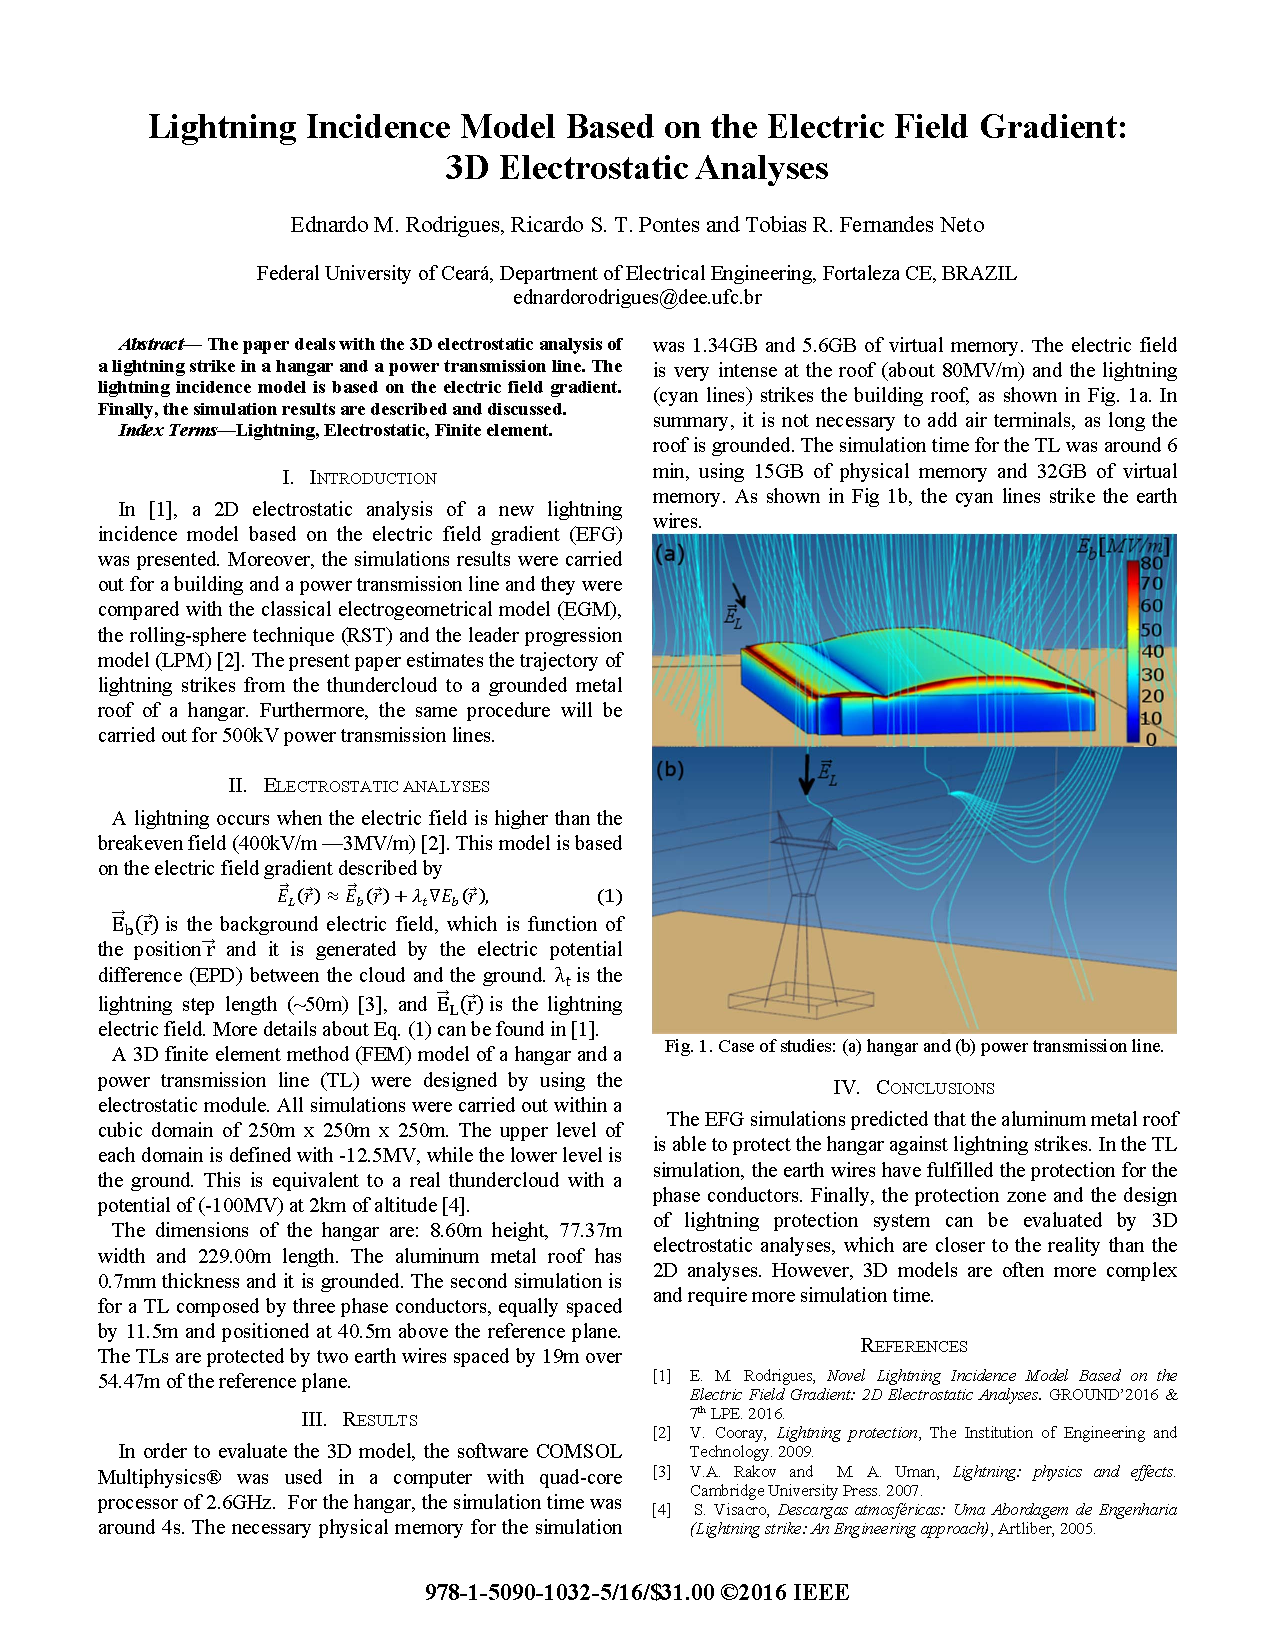
\includepdf[pages={-}]{3-pos-textuais/apendices/PID4416093.pdf}
	\imprimiranexos
		% Adicione aqui os anexos do seu trabalho
		\anexo{Exemplo de um anexo}
\label{an:ex_anexo_a}

Um anexo é um documento que não foi elaborado pelo autor, ou seja, o autor apenas anexa. Anexos podem ser tabelas, mapas, diagramas, \textit{datasheets}, manuais e etc. 




		\anexo{Exemplo de um anexo em PDF}
\label{an:ex_anexo_b}

O autor pode anexar um \gls{PDF}, traduzido como formato portátil de documento. Veja o código fonte utilizado para anexar o arquivo ``Sikasil.pdf'' que foi colocado dentro da pasta ``anexos'' que por sua vez está dentro da pasta ``elementos-pos-textuais''. Tenha muita atenção na hora de especificar o local do arquivo. Recomenda-se não utilizar caracteres especiais para nomear pastas e, principalmente, arquivos. 

Pode-se fazer uma descrição sucinta do arquivo anexado.

%Comando para incluir um arquivo em PDF:
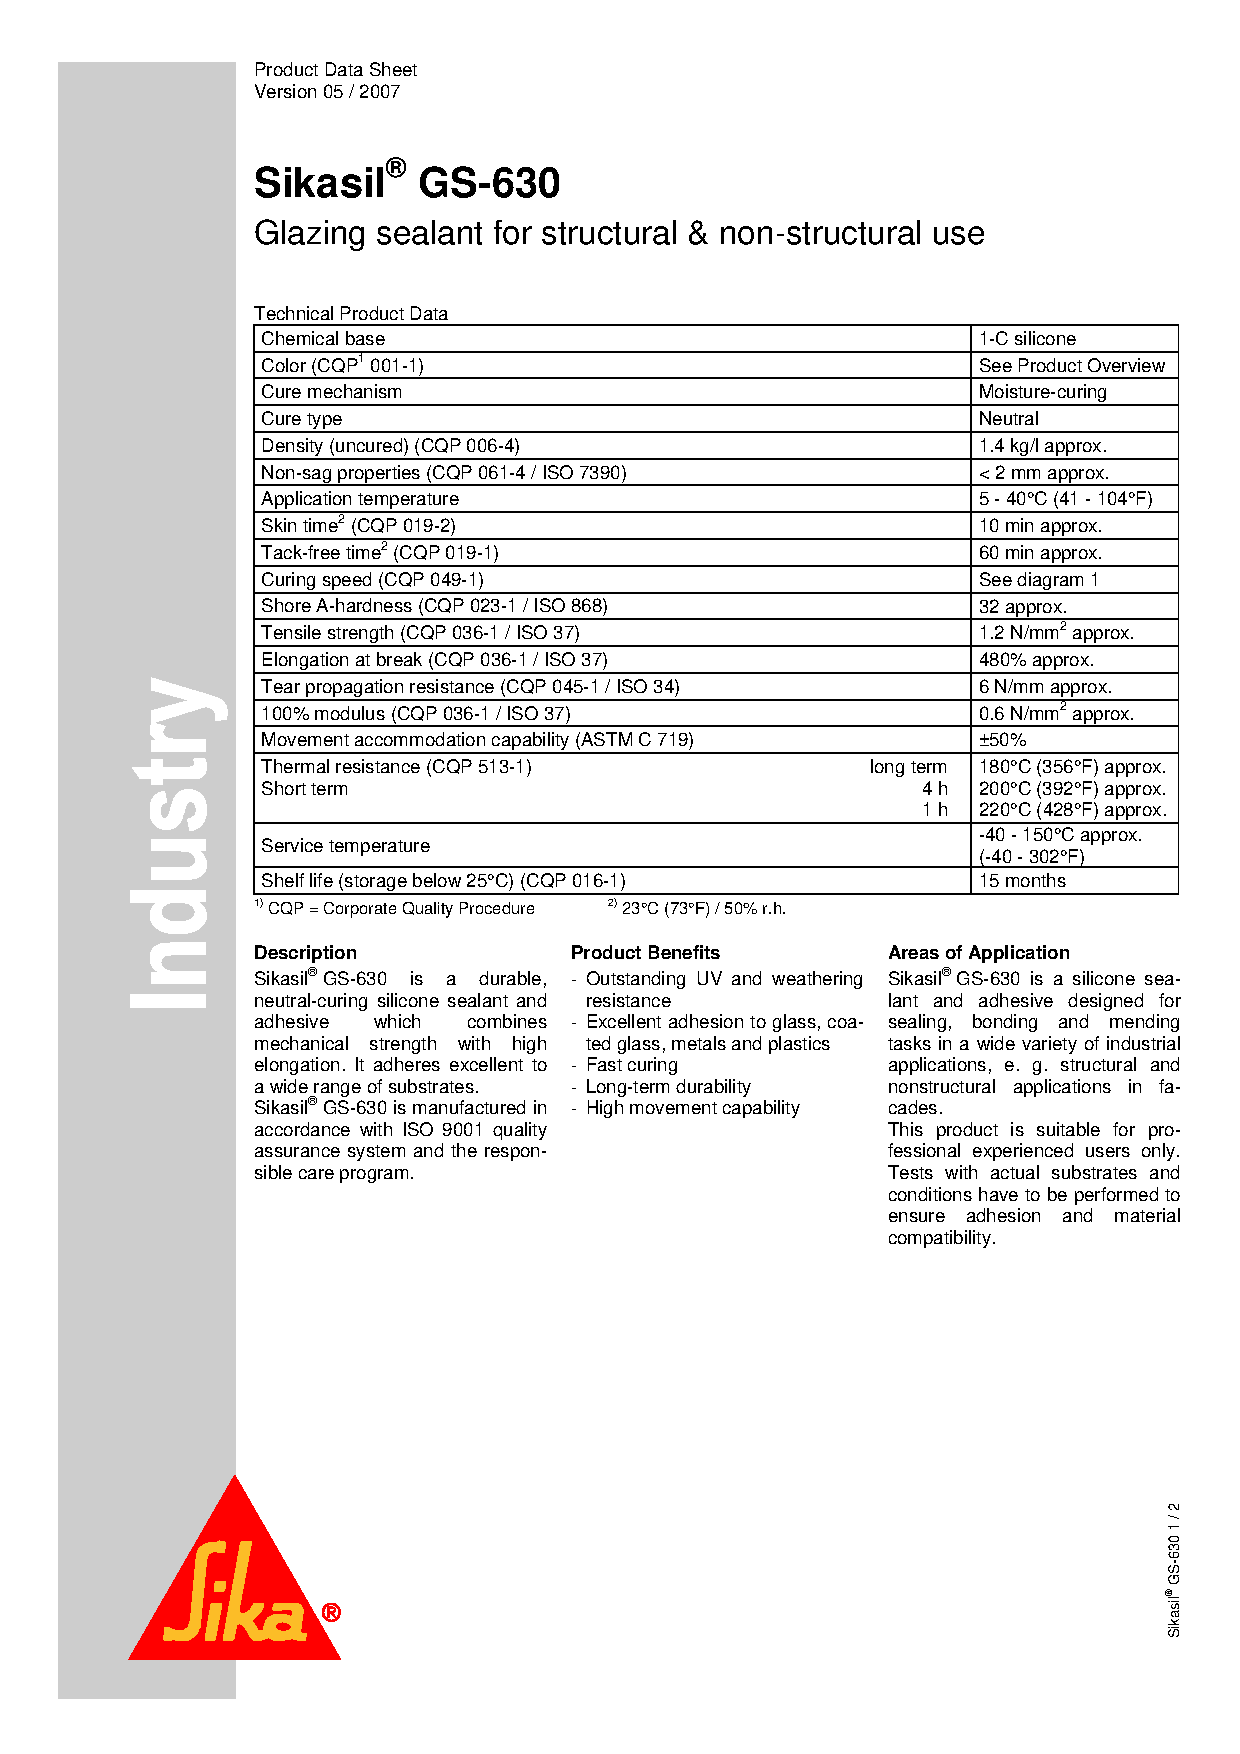
\includepdf[pages={-}]{3-pos-textuais/anexos/Sikasil.pdf}

		
	\imprimirindice

\end{document}